\pagestyle{plain}
\label{toc:{reihe}}
\begin{tikzpicture}[remember picture,overlay]
    \node [anchor=west, text width=83mm, align=left ] at ($(current page.center) - (64mm,-100mm)$) {
    \sffamily \textbf{\Large Verteilte Architekturen}};
    \node at ($(current page.center) - (50mm,-73mm)$) {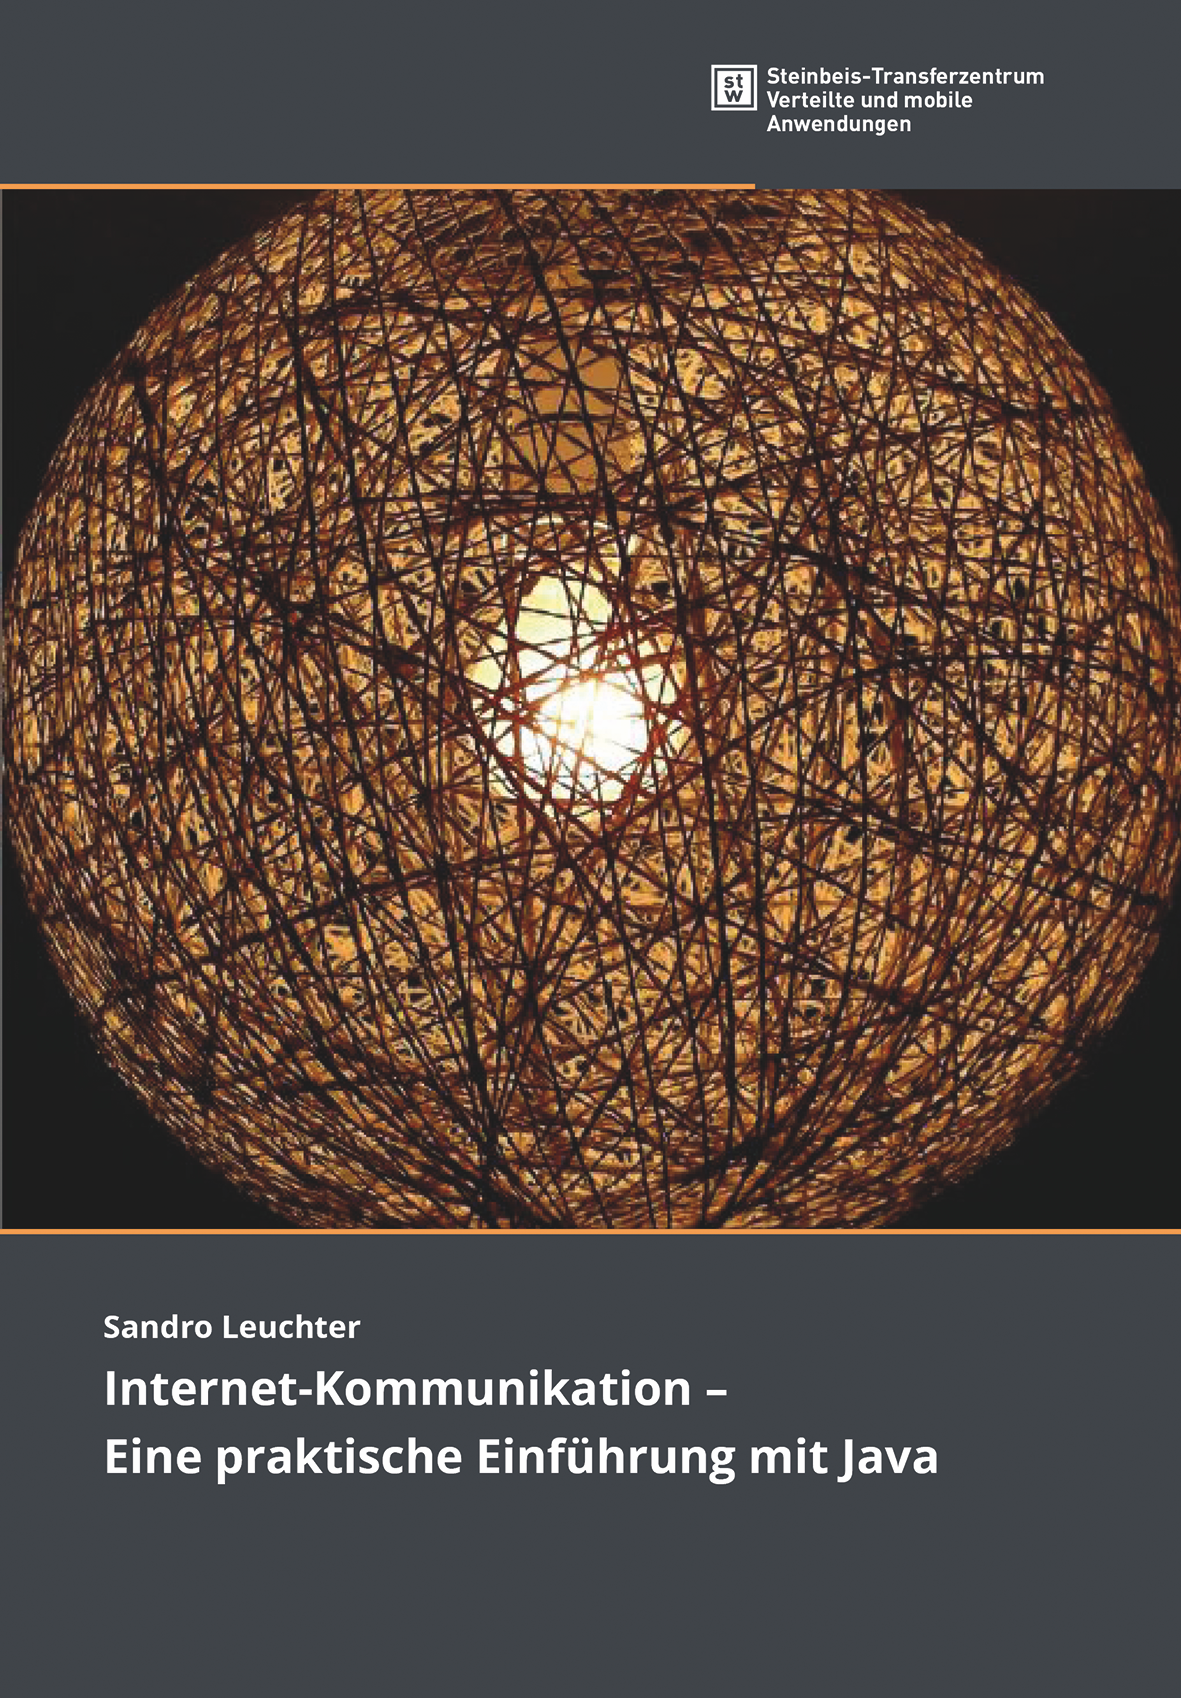
\includegraphics[height=3.5cm]{img/VAR1-Cover.png}};
    \node [anchor=west, text width=83mm, align=left ] at ($(current page.center) - (30mm,-73mm)$) {
    \sffamily\small \textbf{Band 1: Internet-Kommunikation} (2019)
        \begin{itemize}
            \item Internet-Adressierung, DNS, DHCP, UDP, TCP, Socket-Programmierung
            \item Message Broker, JMS, ActiveMQ, MQTT, Paho
            \item Web, HTTP, Servlets, Tomcat, Cloud Computing, Google App Engine
        \end{itemize}};
    \node at ($(current page.center) - (50mm,-36mm)$) {
\includegraphics[height=3.5cm]{img/VAR2-Cover.png}};
    \node [anchor=west, text width=83mm, align=left ] at ($(current page.center) - (30mm,-36mm)$) {
    \sffamily\small \textbf{Band 2: API-Technologien und -Design} (geplant 2020)
        \begin{itemize}
            \item XML, JSON, Protocol Buffers, gRPC, RMI, IDL, WebSockets, XML-RPC, JSON-RPC, SOAP, WSDL
            \item OpenAPI, RESTful Webservices, Webhooks, HATEOAS, CoAP, GraphQL
            \item API Design, Arch.-Bewertung, DDD, API Monitoring/ Analytics, API Gateway
        \end{itemize}};
    \node at ($(current page.center) - (50mm,1mm)$) {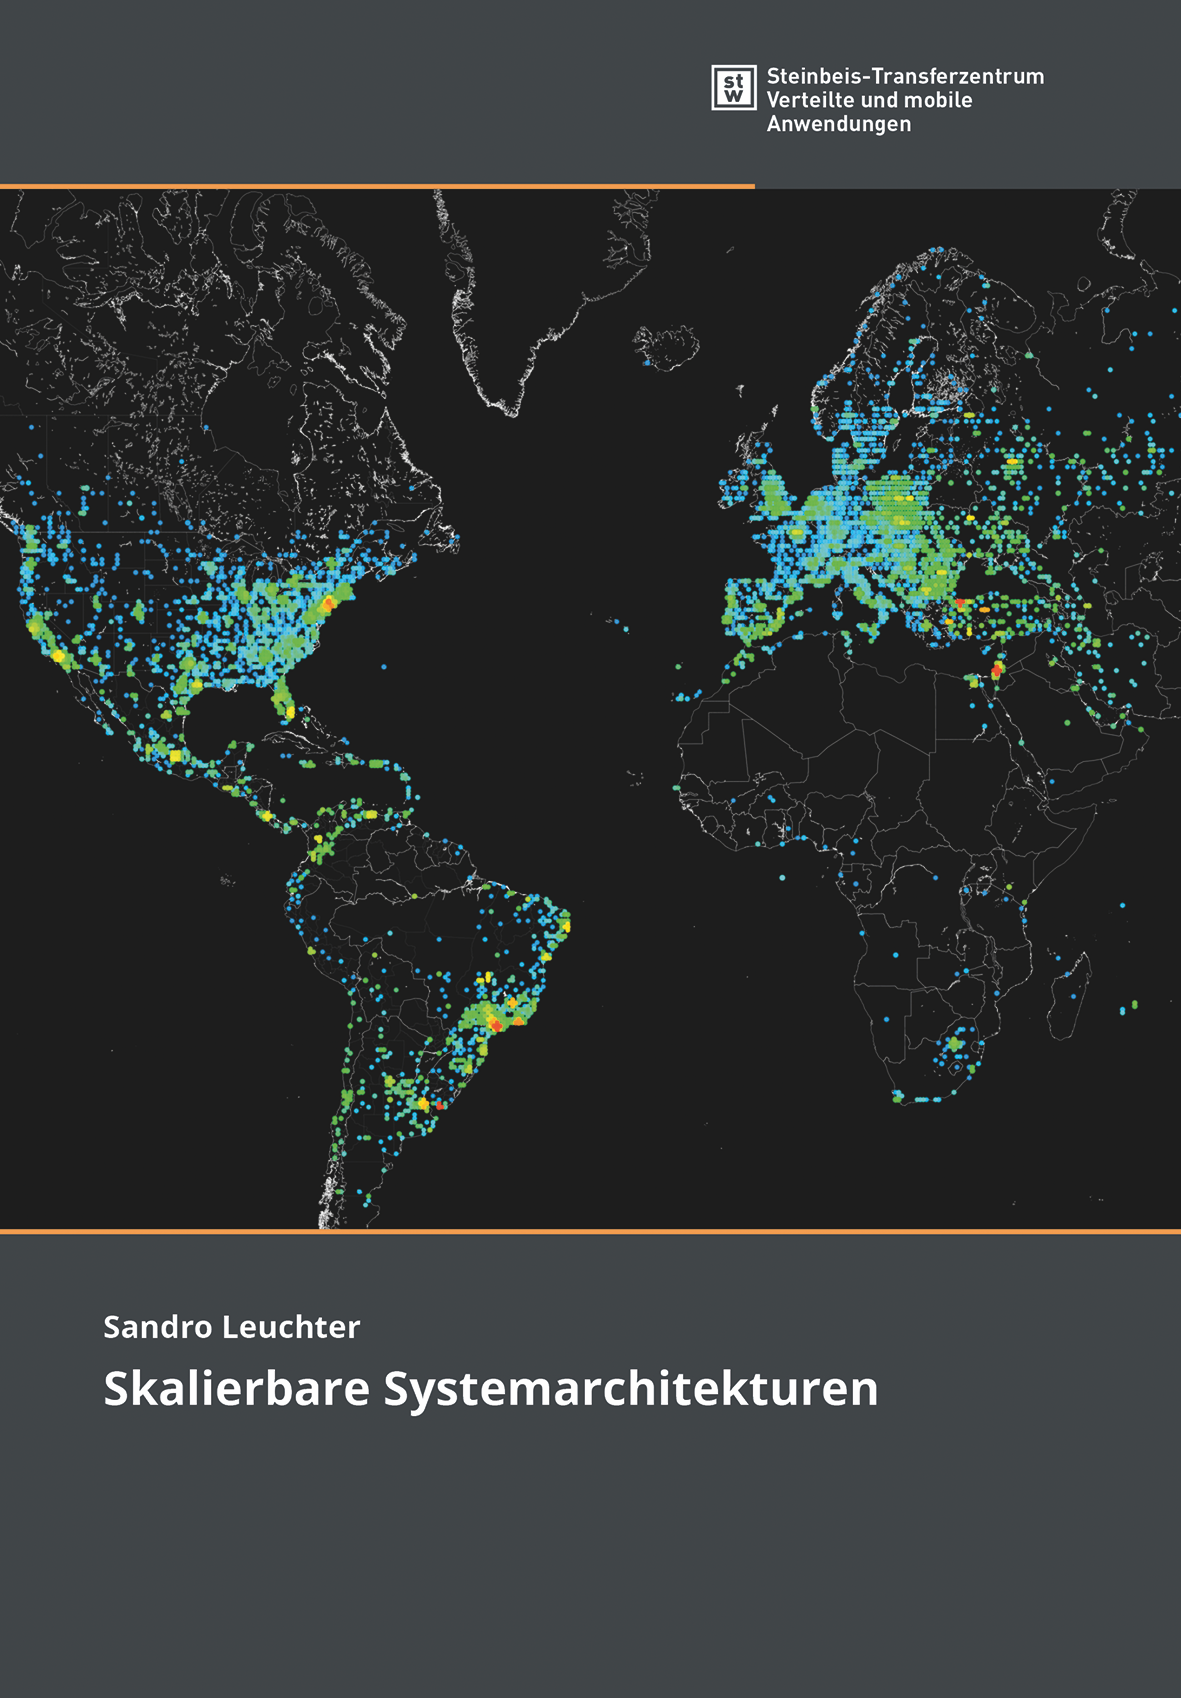
\includegraphics[height=3.5cm]{img/VAR3-Cover.png}};
    \node [anchor=west, text width=83mm, align=left ] at ($(current page.center) - (30mm,1mm)$) {
    \sffamily\small \textbf{Band 3: Skalierbare Systemarchitekturen} (geplant 2021)
        \begin{itemize}
            \item Reaktive Architekturen, Cluster, JGroups, DDS, Kafka, Akka
            \item Microservices, Resource Injection, JNDI, Spring Boot, Spring Cloud, Docker, Kubernetes
            \item Service Discovery, Serverless Architekturen
        \end{itemize}};
    \node at ($(current page.center) - (50mm,38mm)$) {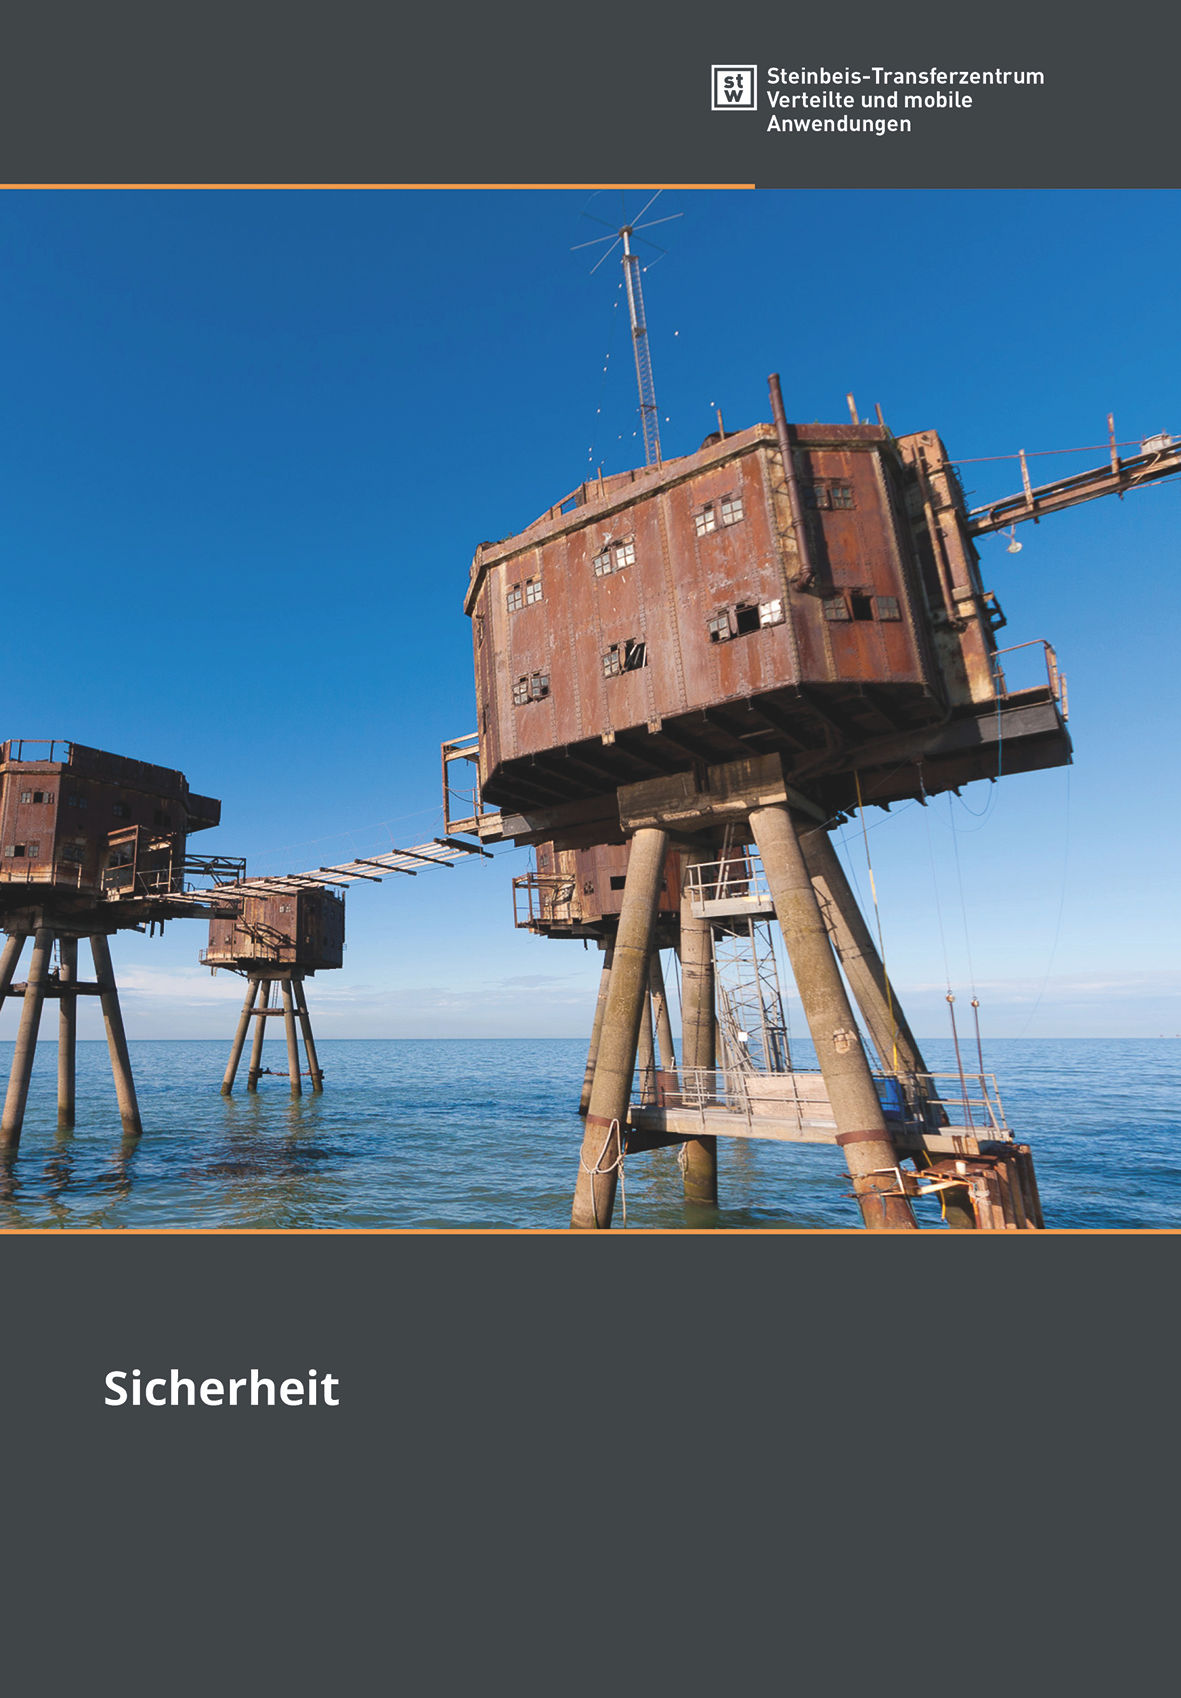
\includegraphics[height=3.5cm]{img/VAR4-Cover.png}};
    \node [anchor=west, text width=83mm, align=left ] at ($(current page.center) - (30mm,38mm)$) {
    \sffamily\small \textbf{Band 4: Sicherheit} (in Planung) 
        \begin{itemize}
            \item Verschlüsselung, PKI, TLS
            \item Authentifizierung, Challenge/Response, HTTP, OAuth, SAML, SSO
            \item Autorisierung, Blockchain
        \end{itemize}};
    \node at ($(current page.center) - (50mm,75mm)$) {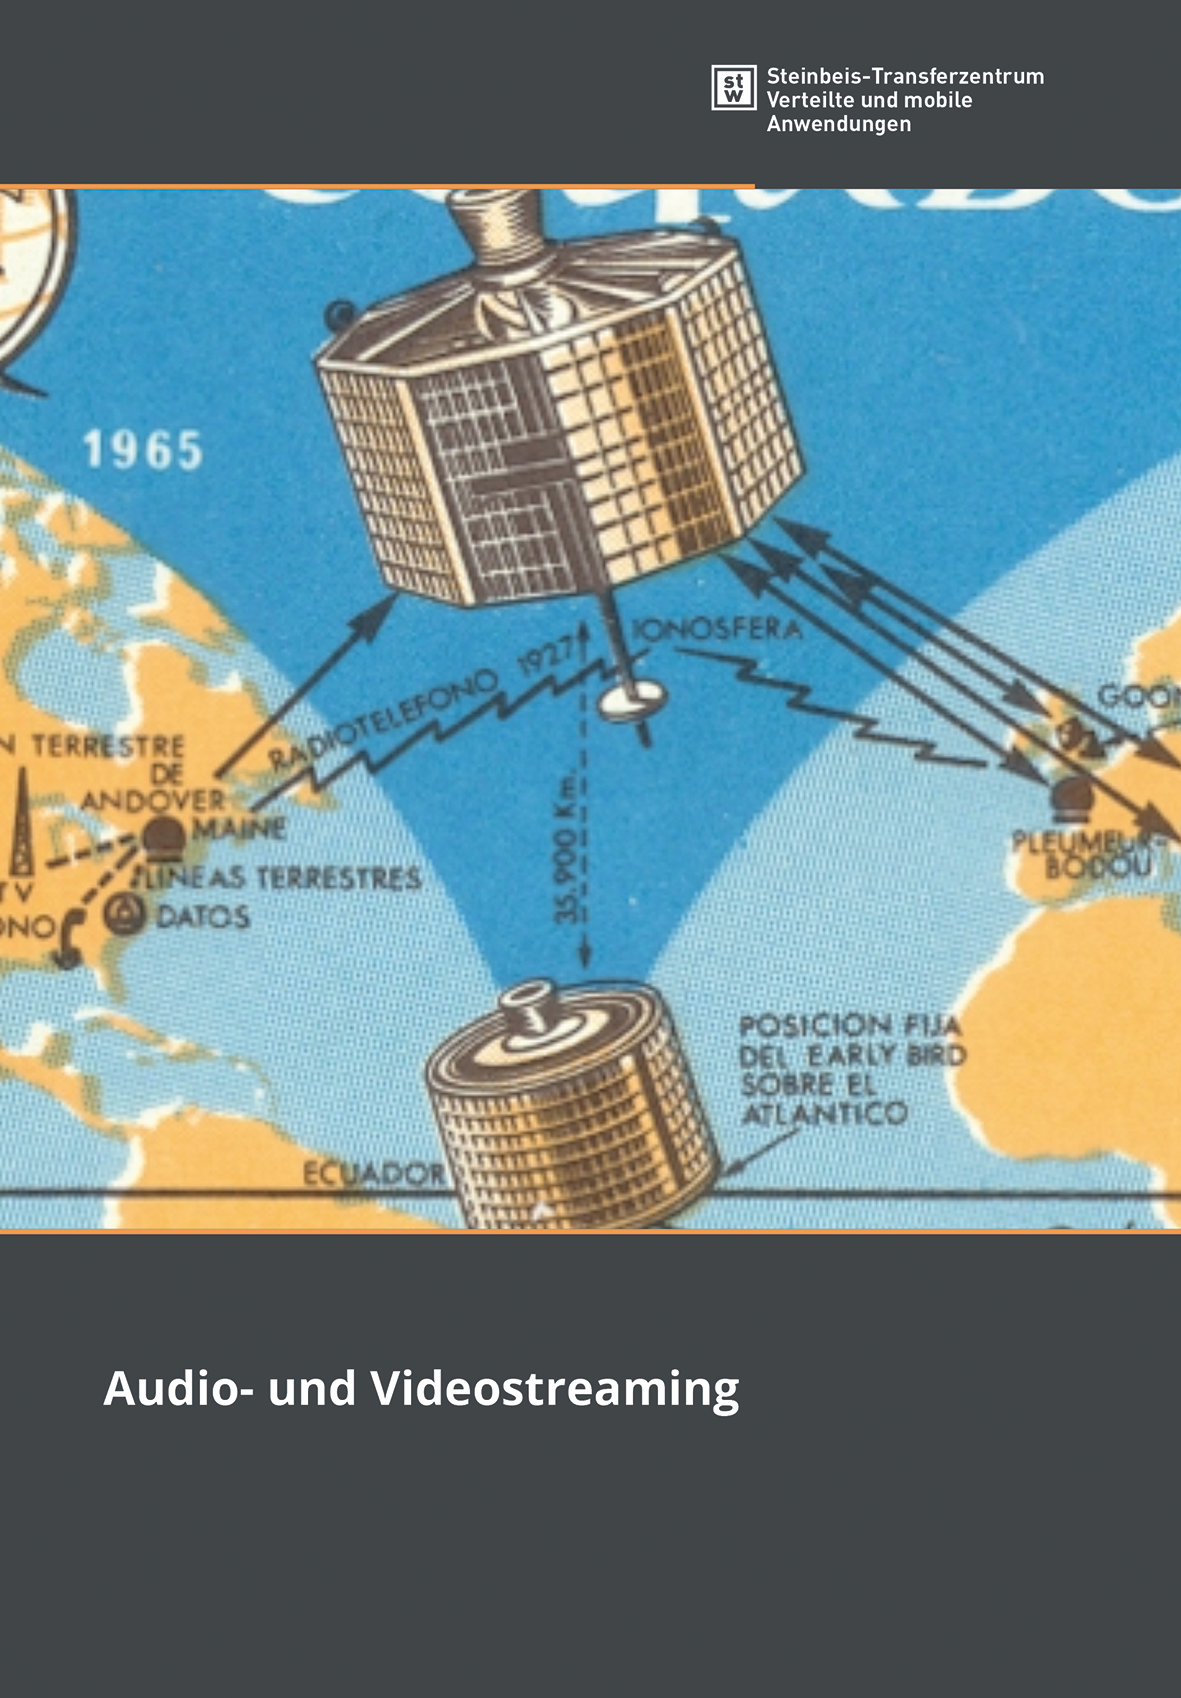
\includegraphics[height=3.5cm]{img/VAR5-Cover.png}};
    \node [anchor=west, text width=83mm, align=left ] at ($(current page.center) - (30mm,75mm)$) {
    \sffamily\small \textbf{Band 5: Audio- und Videostreaming} (in Planung) 
        \begin{itemize}
            \item Disovery: Zeroconf/Bonjour, multicast DNS, UPnP, SSDP, DLNA
            \item On demand  Streaming: Jitter, Live Streaming: RTP, RTCP, RTSP; VoIP: SIP, SIMPLE, WebRTC
            \item Peer to Peer, Streaming Server, multi room, Multicast, Overlay-Netze, CDN
        \end{itemize}};
\end{tikzpicture}